\textbf{Цель работы:}\\
1) измерение давления насыщенного пара жидкости при разной температуре;\\
2) вычисление по полученным данным теплоты испарения с помощью уравнения 
Клайперона-Клаузиуса. \\\indent 

\section*{Теоретические сведения}
Теплоту парообразования вычислим по формуле Клайперона-Клазиуса:
\begin{equation}
    \frac{dP}{dT} = \frac{L}{T(V_2 - V_1)}
\end{equation}
где $V_2 = V$ - объем пара, $V_1$ - объем жидкости.\\\indent
Запишем уравнение Ван-дер-Ваальса для насыщенного пара:
\begin{equation}
    \left ( P + \frac{a}{V^2}\right )(V - b)
\end{equation}
С учетом того, что $b$ и $a$ вносят небольшую погрешность, 
при данных давлениях и температурах можно записать:
\begin{equation}
    V = \frac{RT}{P}
\end{equation}
Однако с учетом того, что $V_1 \ll V_2$ получаем:
\begin{equation}
    L = \frac{RT^2}{P}\frac{dP}{dT} = -R\frac{d(\ln P)}{d(1/T)}
\end{equation}

\section*{Экспериментальная установка}
Экспериментальная установка показана на рисунке ниже. В приборе 13 находится 
исследумая жидкость 14. Давление насыщенных паров определятеся по 
ртутному манометру 15. 
\newpage
\begin{figure}[t!]
    \centering
    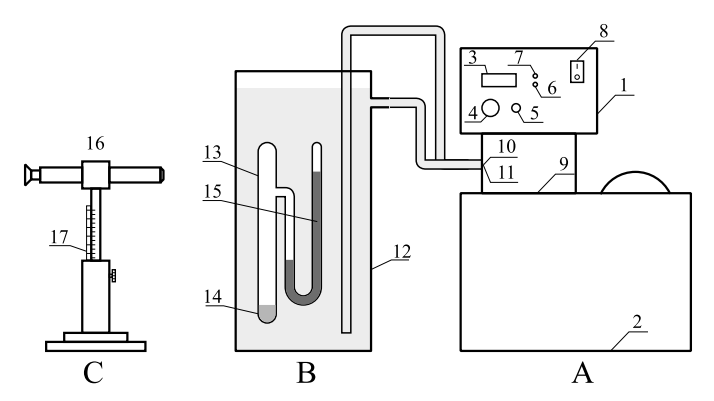
\includegraphics[width=10cm,height=3cm]{setup.png}
    \caption{Схема установки для поределения теплоты испарения}
    \label{fig:setup}
\end{figure}


\section*{Экспериментальные данные}

\begin{table}[h!]
    \centering
    \begin{tabular}{|c|c|c|c|c|c|c|c|c|c|c|c|c|c|c|}
        \hline
        $T^\circ C$ & 23.14 & 24 & 25 & 26 & 27 & 28 & 29 & 30 & 31 & 32 & 33 & 35 & 37 & 40 \\\hline
        $P$, мм.рт.ст & 17.35 & 18.3 & 13.9 & 24.55 & 21.5  & 23 & 24.25 & 25.6 & 27.8 &
        29.7 & 32 & 36.3 &  41 & 48.55\\\hline 
    \end{tabular}
    \caption{Зависимость $P$ от $T$ при нагревании жидкости}
    \vfill 
    \begin{tabular}{|c|c|c|c|c|c|c|c|c|}
        \hline
        $T^\circ C$ & 37 & 35.75 & 34 & 32 & 30 & 28 & 26 & 24\\\hline
        $P$, мм.рт.ст & 44.05 & 46.6 & 37.45 & 33.3 & 29.2 & 26 & 22.8 & 19.6\\\hline
    \end{tabular}
    \caption{Зависимость $P$ от $T$ при охлаждении жидкости}
\end{table}
$$\sigma_{P} = 0.5\text{ мм; }\sigma_{T} = 0.01 \text{ K}$$\\\indent

\begin{figure}[h!]
    \centering
    \begin{figure}{0.45\linewidth}
        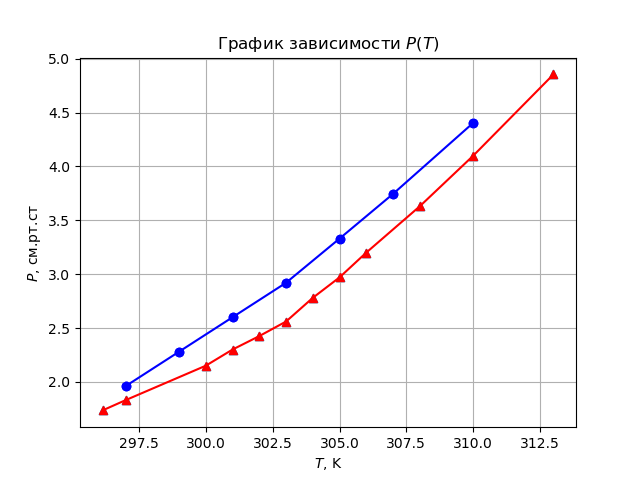
\includegraphics[width=8cm, height=8cm]{simpleplot.png}
        \caption{Зависимость $P$ от $T$ при нагревании жидкости}
    \end{figure}
    % \hfill
    \begin{fiure}
        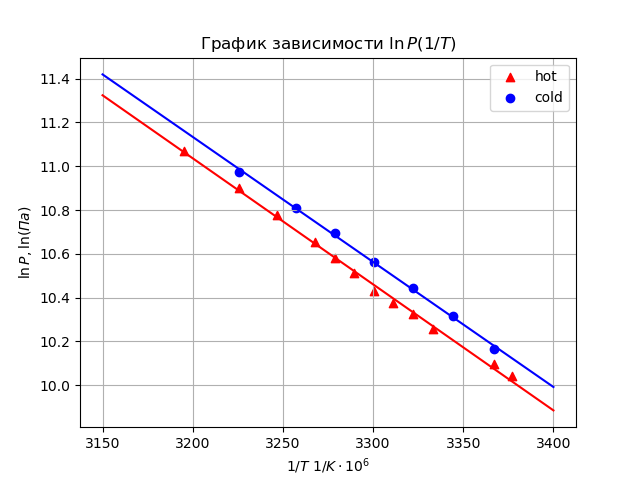
\includegraphics[width=8cm, height=8cm]{complexplot.png}
        \caption{Зависимоть $\ln(P)$ от $\frac{1}{T}$}
    \end{fiure}
\end{figure}

